% Physics Homework Template
% Useful for completing homework questions from the textbook.
\documentclass[11pt]{homework}
\usepackage{siunitx}
\usepackage{amsmath}
\usepackage{tikz}
\usepackage{pgfplots}
\pgfplotsset{compat=1.18}

\newcommand{\hwname}{Corbin Hibler}
\newcommand{\hwemail}{c-hibler@onu.edu}
\newcommand{\hwtype}{Ch. 7 HW}
\newcommand{\hwnum}{}
\newcommand{\hwclass}{PHYS 2311}
\newcommand{\hwlecture}{0}
\newcommand{\hwsection}{Z}

\begin{document}
\maketitle

% MisConceptual Questions
\renewcommand{\questiontype}{MisConcQ}
\setcounter{questionCounter}{0}

\question
1. d\\
3. e\\
5. d\\
7. c\\
9. b\\
11. b\\
13. d

% Problems
\renewcommand{\questiontype}{Problem}
\setcounter{questionCounter}{0}

% Problem 1
\question
\[    
W= \vec{F_g}\cdot\Delta \vec{x}
\]\[
F_g = mg 
\]\[
W = mg \Delta x  = (280)(9.8)(3.80) = \boxed{\qty{10400}{J}}
\]

% Problem 2
\question
\[
W = \vec{F}\cdot \Delta\vec{x}
\] \[
\Delta x = \frac{W}{F_g} = \frac{W}{mg} = \frac{70.0}{(1.85)(9.8)} = \boxed{\qty{3.86}{m}}
\]

% Problem 5
\setcounter{questionCounter}{4}
\question
\[
m = \qty{46.0}{kg}, \quad \Delta x = \qty{10.3}{m}, \quad \mu_k = 0.40
\]\[
W = \vec{F}\cdot \Delta\vec{x}
\]\[
\vec{F}=F_{app} - f_k = 0
\]\[
f_k = F_N\mu_k = mg\mu_k = (46.0)(9.8)(0.40) = \qty{180.32}{N}
\] \[
\implies F_{app} = \qty{180.32}{N}
\]\[
W = (180.32)(10.3) = \boxed{\qty{1860}{J}}
\]
% Problem 8
\setcounter{questionCounter}{7}
\question
\[
    m = \qty{950}{kg}, \quad \Delta x = \qty{510}{m}, \quad \theta = \qty{9.0}{\degree}
\]\[
F_g=mg \sin \theta
\]\[
W = mg \sin \theta \Delta x
\]
\[
    W = (950)(9.8)\sin(9.0)(510) = \boxed{\qty{7.4e5}{J}}
\]
% Problem 12
\setcounter{questionCounter}{11}
\question
\[
\vec x(t)=\vec x_0+\vec v_0t+\frac{1}{2}\vec at^2
\]\[
    \Delta x = \frac{1}{2}at^2 
\]\[
F = ma
\]
\[
    W = F\Delta x = \frac{1}{2}a^2t^2m = \frac{1}{2}(2.0)^2(8.0)^2(4.0) = \boxed{\qty{512}{J}}
\]

% Problem 18
\setcounter{questionCounter}{17}
\question
\[
    \vec{A} \cdot \vec{B} = (2.0x^2)(11.0) + (-4.0x)(2.5x) + (5.0)(0) 
\]
\[
    = 22x^2 - 10x^2 = \boxed{12x^2 \text{ units}}
\]

% Problem 20
\setcounter{questionCounter}{19}
\question
\[
    \vec{A} \cdot \vec{B} = (5.8)(8.2) + (-3.4)(4.3) + (-6.2)(-7.0) = 76.34
\]\[
|\vec{A}| = \sqrt{(5.8)^2+(-3.4)^2+(-6.2)^2} = 9.15
\]\[
|\vec{B}| = \sqrt{(8.2)^2+(4.3)^2+(-7.0)^2} = 11.61
\]\[
\theta = \arccos\left(\frac{A \cdot B}{|A||B|}\right) 
\]
\[
    \theta = \arccos\left(\frac{76.34}{9.15 \cdot 11.61}\right) = \boxed{\qty{44.2}{\degree}} 
\]

% Problem 22
\setcounter{questionCounter}{21}
\question
\[
    \vec{V_1} = 0 \hat{i} + 75 \hat{k}
\]
\[
    \vec{V_2} = 48\cos(-48) \hat{i} + 48\sin(-48) \hat{k} = 32.11 \hat{i} - 35.67 \hat{k}
\]
\[
    \vec{V_1} \cdot \vec{V_2} =  (0)(32.11) + (75)(-35.67) = \boxed{\qty{-2675}{units}}
\]

% Problem 25
\setcounter{questionCounter}{24}
\question
\begin{alphaparts}
\questionpart
\[
    \vec{B} + \vec{C} = (-8.0 + 5.8)\hat{i} + (6.1-9.2)\hat{j} + 4.2 \hat{k} = -2.2 \hat{i} -3.1 \hat{j} +4.2 \hat{k}
\]
\[
    \vec{A} \cdot (\vec{B}+\vec{C}) = (9.0)(-2.2) + (-8.5)(-3.1) + (0)(4.2) = \boxed{6.55}
\]
\questionpart
\[
    \vec{A}+\vec{C} = (9.0+5.8)\hat{i} + (-8.5-9.2)\hat{j} = 14.8\hat{i} - 17.7 \hat{j}   
\]\[
\vec{B} \cdot (\vec{A}+\vec{C}) = (-8.0)(14.8) + (6.1)(-17.7) + (4.2)(0) = \boxed{-226}
\]
\questionpart
\[
    \vec{B}+\vec{A} = (-8.0+9.0)\hat{i} + (6.1-8.5)\hat{j} + (4.2+0)\hat{k} = 1\hat{i} - 2.4 \hat{j} + 0\hat{k}
\]
\[
    (\vec{B}+\vec{A}) \cdot \vec{C} = (1)(5.8) + (-2.4)(-9.2) + (0)(0) = \boxed{27.9}
\]


\end{alphaparts}

% Problem 37
\setcounter{questionCounter}{36}
\question

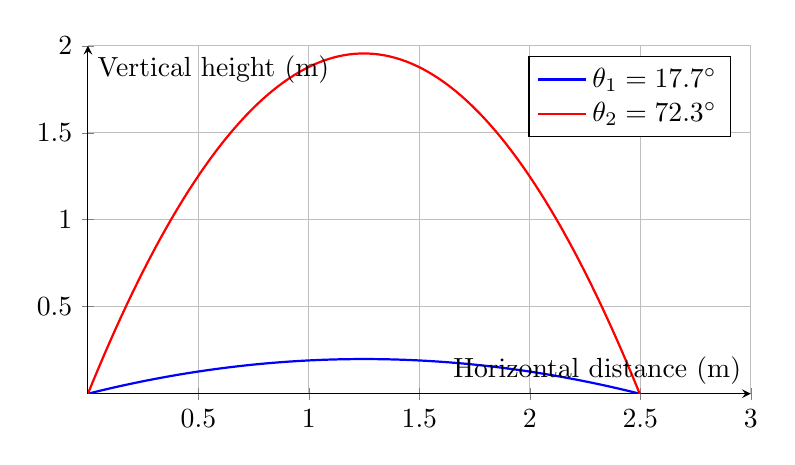
\begin{tikzpicture}
\begin{axis}[
    xlabel={Horizontal distance (m)},
    ylabel={Vertical height (m)},
    axis lines=middle,
    grid=both,
    xmin=0, xmax=3, % Adjust as necessary for better fit
    ymin=0, ymax=2, % Adjust as necessary
    samples=100,
    legend pos=north east,
    width=10cm, height=6cm
]

% Parameters
\pgfmathsetmacro{\v}{6.5} % initial velocity in m/s
\pgfmathsetmacro{\g}{9.8} % gravity in m/s^2

% First trajectory (theta1 = 17.7 degrees)
\pgfmathsetmacro{\thetaone}{17.7}
\addplot[
    domain=0:2.5, 
    thick, 
    blue, 
]
{ x*tan(\thetaone) - (\g/(2*\v^2*cos(\thetaone)^2)) * x^2 };
\addlegendentry{$\theta_1 = 17.7^\circ$};

% Second trajectory (theta2 = 72.3 degrees)
\pgfmathsetmacro{\thetatwo}{72.3}
\addplot[
    domain=0:2.5, 
    thick, 
    red, 
]
{ x*tan(\thetatwo) - (\g/(2*\v^2*cos(\thetatwo)^2)) * x^2 };
\addlegendentry{$\theta_2 = 72.3^\circ$};

\end{axis}
\end{tikzpicture}


\end{document}
